% https://www.naept.com/en/blog/validation-plan-check-your-product-meets-the-customer-needs-part-one/
\setchapterpreamble[u]{\margintoc}
\chapter{Validation Plan\\Check your product meets the customer needs}
\label{sec:ValidationPlan}

We’ll see how to build a validation plan ensuring your product is matching all your customer’s requests.

\section{What is it used for?}

The more complex products you create, the more difficult it is to check they fit all the customer’s specifications. In the chapter ~\ref{TraceabilityMatrices}, we talked about the traceability matrices, the dependency connections between the customer’s need and your product’s features can be numerous! And when you deliver your product (or your service), you have to be sure that all those features are correctly working.

Besides, sometimes a new feature request happens and challenges all the work previously done: “Now the car must carry 7 people, not just 5”. “OK so the car must be longer, the engine stronger…”. Those evolutions shall not alter what was correctly working earlier. To validate this point we have to perform “regression tests”.

This is why creating a list of test checking that each and every feature works correctly with the other is crucial. Such a list is what we call a validation plan.

\section{What does it look like?}
Depending on the complexity of you project, the way you describe your tests can takes different shapes: from a very light one to the most bullet-proof. We have identified 3 ways:

\subsection{1. In the same document than your product’s specifications}

\begin{figure}[h]
    \centering
    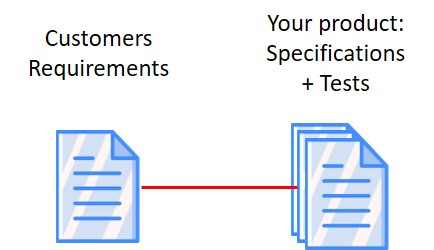
\includegraphics[]{1-in-the-same-document.jpg}
    \caption{The product specifications and tests are in the same document}
    \label{fig:SameDocument}
\end{figure}

Your customer has described his need in a requirements document. You reply to it in a specifications document where you explain all the features of you future product. Each of those features is followed by a corresponding test with a status checkbox telling if it is OK or not.

Like this you reduce the number of documents by gathering everything in one.

But if the project grows and the product requires more complex features, you may want to test several of them at once if you can. This format doesn’t allow this kind of test management: you cannot “factorize” the tests and therefore you may have redundancies. Which is not very efficient.

\subsection{2. List the tests in a separate document}

\begin{figure}[h]
    \centering
    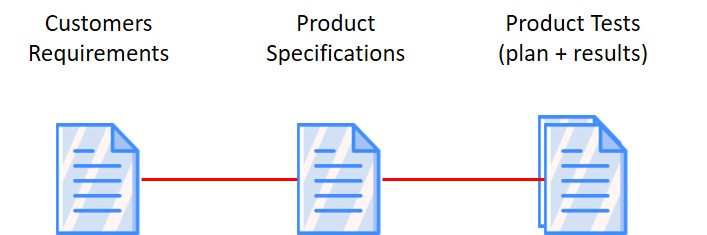
\includegraphics[]{2-in-two-document.jpg}
    \caption{Tests in their own document}
    \label{fig:TwoDocument}
\end{figure}

Your customer has described his needs in a requirements document. You reply to it in a specifications document. And you describe the tests on those specifications in a third document. Each test can have specific fields to precise details on the results (measured values, expected results, status, comments…).

The benefit is that you can now factorize the tests: in one bigger test you can check the validity of several specifications at once and reduce the time spent on this activity.

The drawback is now you have to keep track of the links between the specifications and their tests. But it is easy to do so with traceability matrices.

Now, a new hidden problematic comes out. It only occurs if you have to perform your tests several times. Let’s take a concrete example. Imagine you are a reusable anti-COVID masks manufacturer (not the disposable ones). So you deliver lots of masks, all the same, and you have to test each and everyone of them before to put them on the market. For each mask you have to duplicate the test document to perform the campaign, and to fill it with the mask tests results but the test descriptions are exactly the same. That makes a lot of redundancy between the 2 documents. Let’s see how to optimize this…

\subsection{3. Cut the test document in 2: the procedures and the results}

\begin{figure}[h]
    \centering
    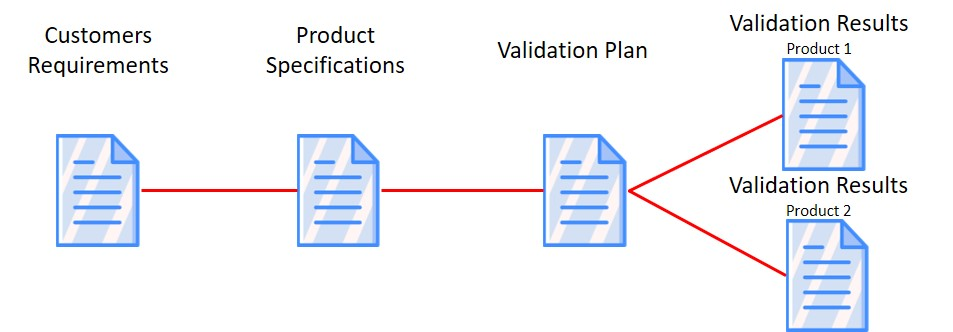
\includegraphics[]{3-in-three-documents.jpg}
    \caption{Test procedures and results in 2 documents}
    \label{fig:ThreeDocument}
\end{figure}

Here is the best way to do, from our point of view:

\begin{itemize}
    \item The tests procedures are detailed in a first document: the validation plan
    \item All the results for the same product are gathered in its own document: the validation results
\end{itemize}

OK the obvious drawback is the multiplication of the documents. From “one doc to rule them all” we go to at least 3 (specifications, validation plan and validation results) and more if you deliver several identical products. And off-course you have to manage a traceability matrix for each document relation (red link).

BUT,

it is the best way for us because of the following reasons:

\begin{itemize}
    \item Each document deals with only one aspect of the project: specifications design the solution, validation plan builds the tests, validation results report the status on the product.
    \item Each document is therefore shorter and so easier to maintain up to date.
    \item Consequently, each document can evolve independently from the other one. And if there is an impact, the traceability matrices will tell you exactly where.
\end{itemize}

In the following sections, we will explain the organizations of the validation plan and results in two separated document. But even if they are merged it works the same.

\section{The procedures}
In the validation plan you will define all the procedures for the required tests to validate that your product correctly matches its specifications.

The validation plan will contain enough tests if and only if all of the specifications are covered by one test at least. Although it doesn’t mean there should be one test for each specification. And this is one major benefit of the validation plan, you can do:

\begin{itemize}
    \item one test for one specification
    \item one test for several specifications at once
    \item several tests to check only one complex specification
\end{itemize}

That’s why traceability matrices are very useful! By tracking all those relations they ensure at least one test covers each specification. If it is not the case, you know you need more tests and what to do them on.

\section{How to structure a test procedure?}
